\section{Stereoskopische Analyse des Krebsnebels}
\label{sec:analyse}

\subsection{Datenselektion und -rekonstruktion}

Abbildung~\ref{fig:analysischain} zeigt den typischen Ablauf einer
stereoskopischen Analyse mit MAGIC Daten. Die hierzu verwendeten Programme sind
eingebettet in das Softwarepaket MARS (MAGIC analysis and reconstruction
software). In einem ersten Schritt durchlaufen die
Rohdaten der beiden Teleskope eine \textbf{Vorprozessierung}. Dazu gehören die
Zeit- und Ladungskalibrierung der einzelnen Pixel der Kamera mit dem Programm
\textit{sorcerer}, sowie das Image Cleaning und die Parametrisierung des
Kamerabildes mit dem Programm \textit{star}. Beim Image Cleaning wird Rauschen
aus dem Kamerabild entfernt, indem nur die Pixel der Kamera berücksichtigt
werden, die eine bestimmte Signalstärke gemessen haben. Dabei ist die geforderte
Signalstärke auch davon abhängig, ob Pixel in direkter Nachbarschaft
berücksichtigt worden sind. Nach der Reinigung des Kamerabildes kann das
Schauerbild durch eine Ellipse beschrieben werden, die durch Größen, wie zum
Beispiel den Schwerpunkt, die Länge und Breite und den Abstand des Schwerpunktes
zum anvisierten Ziel parametrisiert wird. Im Anschluss daran werden die Daten
der Teleskope durch die Software \textit{superstar} kombiniert und
Stereoparameter für die weitere Analyse berechnet.

\begin{figure}[H]
  \centering
  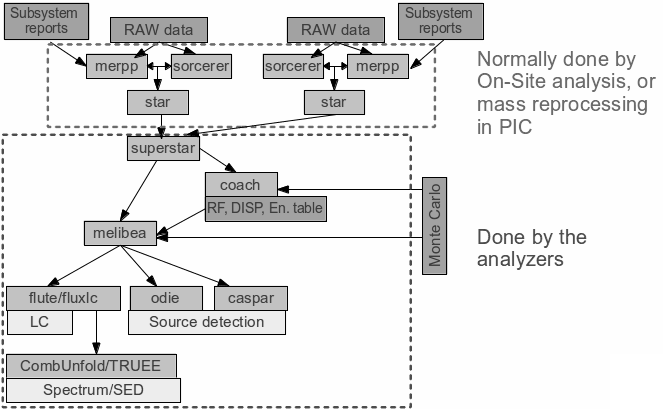
\includegraphics[width=0.9\textwidth]{figures/analysischain.png}
  \caption{Ablauf einer typischen stereoskopischen Analyse mit MAGIC Daten. In
  der hier durchgeführten Analyse wurde mit den Programmen \textit{coach},
  \textit{melibea}, \textit{flute}, \textit{odie}, \textit{caspar} und
  \textit{CombUnfold} gearbeitet \cite{magic_wiki}.} % Referenz: MAGIC wiki
  \label{fig:analysischain}
\end{figure}

In einem nächsten Schritt findet die \textbf{Datenselektion} statt. Der Schritt
ist wichtig, um sicherzustellen, dass die verwendeten Daten vergleichbar und
nicht durch äußere Einflüsse verfälscht sind. Somit dient die Selektion der
Qualitätssicherung der Daten. Für die weitere Analyse werden nur Daten
weiterverwendet, die den folgenden Kriterien genügen:
\begin{itemize}
  \item $\SI{5}{\degree}<\text{Zenitwinkel}<\SI{35}{\degree}$
  \item $\SI{-180}{\degree}<\text{Azimuthwinkel}<\SI{360}{\degree}$
  \item Maximale Bewölkung: \SI{35}{\percent}
\end{itemize}
Dabei sind der minimal und maximal zulässige Zenit- bzw. Azimuthwinkel durch die
Begrenzung durch das Teleskop gegeben. Die Schnitte dienen dazu fehlerhafte
Daten herauszufiltern. Die Wahl einer maximalen Bewölkung zum Zeitpunkt der
Messung sichert die Vergleichbarkeit und Qualität der genommenen Daten.

Als nächstes wird das Programm \textit{coach} (Compressed Osteria Alias
Computation of the Hadroness parameter) verwendet, um Modelle für die
\begin{enumerate}
  \item Separation von Gamma- und Hadronenschauern,
  \item Energieabschätzung und
  \item Positionsrekonstruktion
\end{enumerate}
aufzustellen. Dies ist notwendig, um das beobachtete Signal klassifizieren bzw.
rekonstruieren zu können. Die Unterscheidung von Gamma- und Hadronenschauern
erfolgt mit Techniken des \textit{maschine learning}, da die Prozesse in den
Kameras sehr ähnliche Topologien zeigen. Hadronen, die
in die Atmosphäre eindringen wechselwirken sehr wahrscheinlich zunächst hadronisch.
Die entstehenden leichteren Hadronen zerfallen anschließend, bis sich Pionen, also
die leichtesten Hadronen bilden. Dabei fächert sich der Schauer im Vergleich zu
Photonenschauern erheblich auf. Die große Pionenzahl in hadronischen Schauern sorgt
des Weiteren dafür, dass sehr viele Myonen entstehen, welche sich in den Kameras als
kreisrunde Schauer niederschlagen.
Gammaschauer hingegen wechselwirken beinahe ausschließlich elektromagnetisch durch
Streuung sowie Paarbildung. Die Wahrscheinlichkeit für die Paarbildung von Myonen
ist dabei vernachlässigbar gegen die der Bildung von Elektronen. Durch die fehlende
Erzeugung vieler Hadronen sind Gammaschauer außerdem deutlich in Richtung Gesamtimpuls
geboostet. \\
Abbildung~\ref{fig:gamma_hadron} zeigt den Unterschied der Form eines
hadronischen und eines elektromagnetischen Schauers. Zur Klassifikation wird ein
\textit{random forest} verwendet. Dieser wird trainiert mit Off-Daten, die an
einer Stelle am Himmel aufgenommen wurden, an dem kein Signal der Quelle
erwartet wird und somit als Nullmessung dienen und einem Monte Carlo generierten
Datensatz, der auf Grundlage eines Modells generiert wurde, welches durch
Gammastrahlung induzierte Teilchenschauer beschreibt. Um die Trennkraft des
Klassifizierers zu testen wird der Monte Carlo Datensatz zu Beginn in einen
Test- und einen Trainingsdatensatz aufgeteilt. Somit ist es möglich mit einem
Teil des Datensatzes den Klassifizierer zu trainieren und mit dem anderen Teil
zu testen.

\begin{figure}
  \centering
  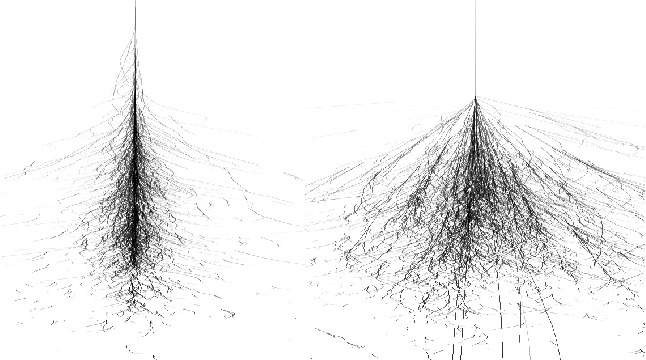
\includegraphics[width=0.7\textwidth]{figures/gamma_hadron.png}
  \caption{Struktur eines elektromagnetischen (links) und eines hadronischen
  (rechts) Schauers. Da Hadronen mit geringer Wahrscheinlichkeit mit der
  Atmospähre wechselwirken als Elektronen und Photonen, fliegen sie weiter und
  der Schauer fächert weiter auf.}
  \label{fig:gamma_hadron}
\end{figure}

Für die Energierekonstruktion werden sogenannte \textit{lookup tables} (LUTs)
generiert, durch die eine Abschätzung der Energie aufgrund der Korrelation
zwischen den Bildparametern und der Stärke des Signals erfolgt.

Nachdem die Modelle erstellt wurden, werden diese mit dem Programm
\textit{melibea} auf den vollständigen Datensatz angewendet. Mit dem nun fertig
präparierten Datensatz können im letzten Analyseschritt Physikresultate
produziert werden.

\subsection{Ergebnisse der Analyse}

Abbildung~\ref{fig:skyplot} (auch \textit{skyplot} genannt) zeigt den mit dem
Programm \textit{caspar} berechneten relativen Fluss aufgetragen gegen die
Position am Himmel. Die eingezeichnete \textit{point spread function} (PSF)
veranschaulicht die Detektorantwort des Teleskops auf eine punktförmige Quelle
am Himmel und ist somit ein Maß für die Auflösung des Teleskops. Es zeigt sich,
dass der Krebsnebel für das Teleskop eine Punktquelle darstellt.

\begin{figure}[H]
  \centering
  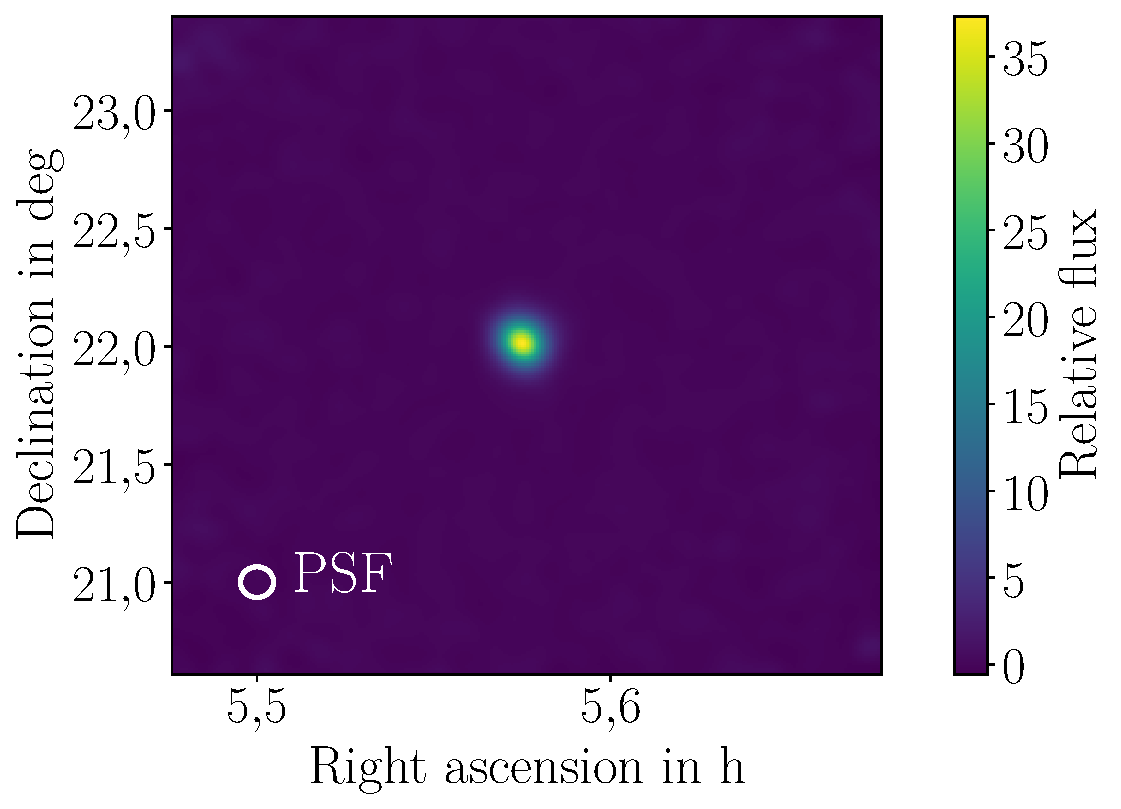
\includegraphics[width=0.8\textwidth]{figures/caspar_flux_skymap.pdf}
  \caption{Veranschaulichung des relativen Flusses in Abhängigkeit von der
  Position am Himmel. Die eingezeichnete Ellipse stellt die
  \textit{point spread function} (PSF) dar und ist ein Maß für die Auflösung des
  Teleskops.}
  \label{fig:skyplot}
\end{figure}

Abbildung~\ref{fig:detectionplot} zeigt den sogenannten \textit{detection plot}.
Hierbei ist die Anzahl der detektierten Photonen aufgetragen gegen den Abstand
zur anvisierten Position. Als Maß für den Abstand wird typischerweise
der eingeschlossene Winkel $\theta$ zum Quadrat gewählt, unter dem relativ zur
anvisierten Position gemessen wird. Es zeigt sich ein stark von Null
abfallender Verlauf. Zur Erstellung der Abbildung wurde das Programm
\textit{odie} verwendet. In einem nächten Schritt kann nun die Signifkanz der
Quelle über dem gemessenen Untergrund bestimmt werden. Dabei wird der Schnitt
auf $\theta^2$ so gewählt, dass die Signifikanz maximiert wird. Es ergibt sich
eine erwartete hohe Signifikanz von $\num{69.83}\sigma$ mit einem $\theta^2$
Schnitt sehr nahe bei Null, wodurch die Punktförmigkeit der Quelle für das
Teleskop nochmal deutlich wird.

\begin{figure}[H]
  \centering
  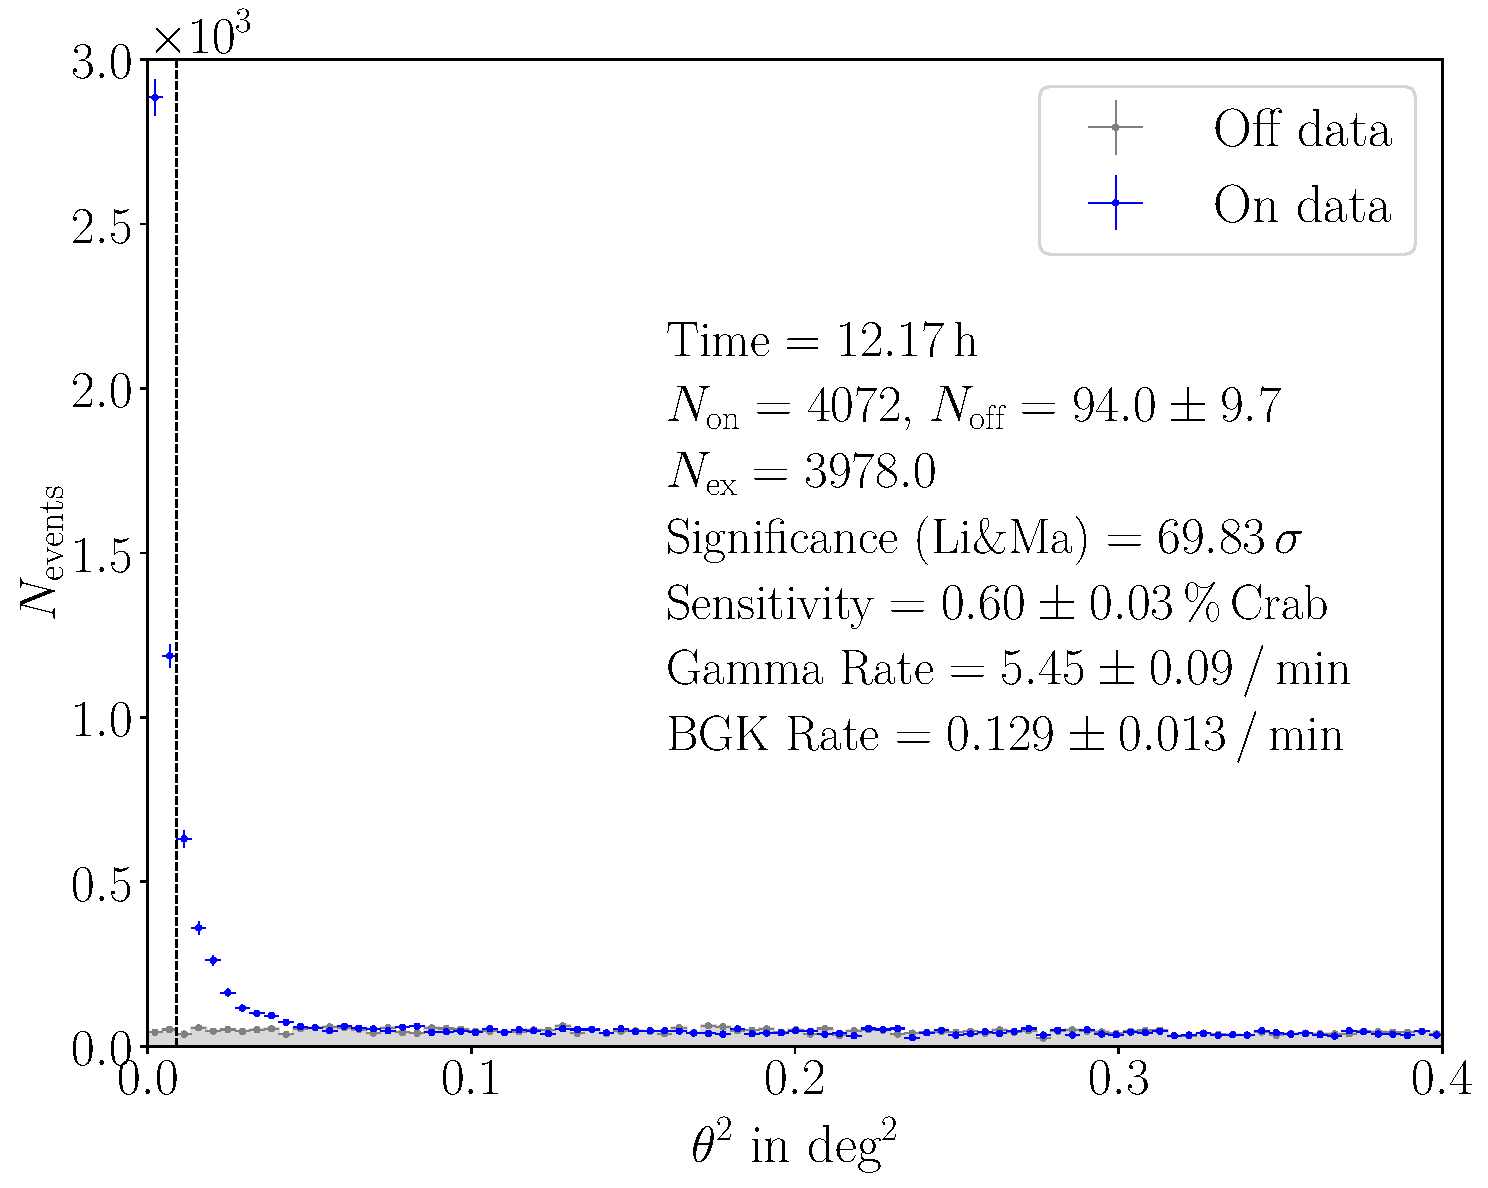
\includegraphics[width=0.8\textwidth]{figures/odie_thetasquared.pdf}
  \caption{Anzahl gemessener Photonen in Abhängigkeit vom Abstand zum
  Quellmittelpunkt. Es zeigt sich eine hohe Signifikanz der Quelle über dem
  gemessenen Untergrund.}
  \label{fig:detectionplot}
\end{figure}

Der mit der Software \textit{flute} berechnete Fluss von Photonen mit einer
Energie größer als \SI{300}{\giga\electronvolt} aufgetragen gegen den
Beobachtungszeitpunkt ist in der sogennaten Lichtkurve in
Abbildung~\ref{fig:lichtkurve} zu sehen. Es zeigt sich, dass der gemessene Fluss
zu allen Zeitpunkten im Rahmen der Fehler nicht signifikant vom zeitlichen
Mittelwert abweicht. Schwankungen zwischen den gemessenen Werten können
auch durch unterschiedliche Randbedingungen, wie zum Beispiel das Wetter erklärt
werden; unterschiedlich große statistische Fehler der Werte durch
unterschiedlich lange Beobachtungszeiträume und damit einhergehender
unterschiedlicher Datenmengen. Längere Zeiträume ohne Messpunkte können dadurch
erklärt werden, dass der Krebsnebel im Zeitraum November / Dezember an einem für
das MAGIC Teleskop nicht sichtbaren Teil des Nachthimmels steht.

\begin{figure}
  \centering
  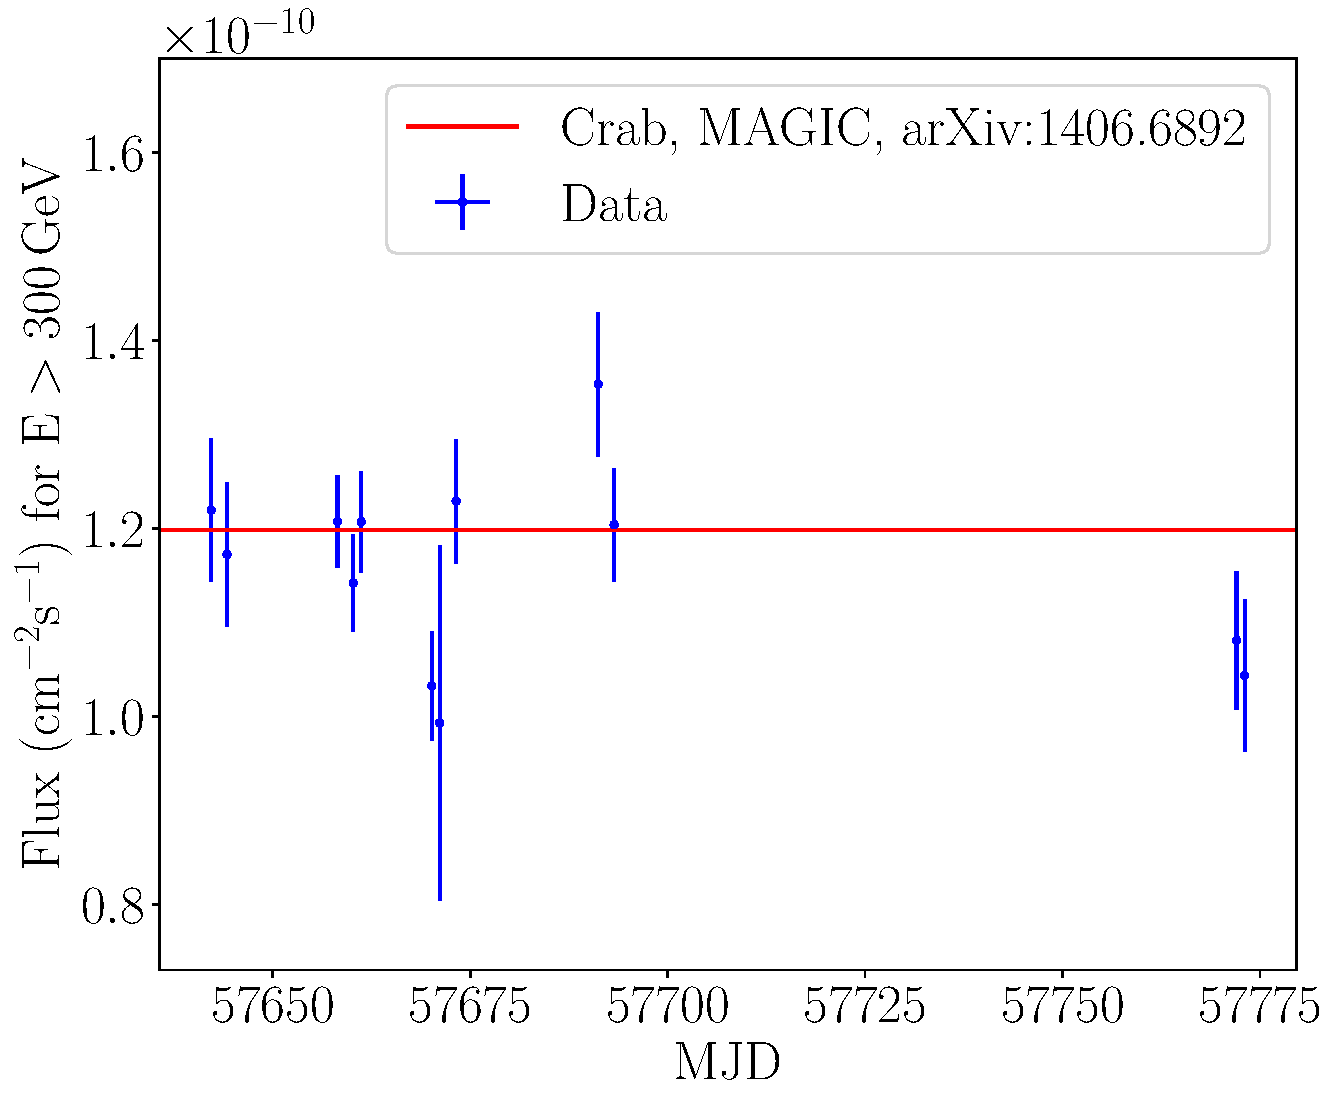
\includegraphics[width=0.8\textwidth]{figures/flute_lichtkurve.pdf}
  \caption{Fluss von Photonen mit Energien größer als
  \SI{300}{\giga\electronvolt} aufgetragen gegen den Beobachtungszeitpunkt. Eine
  gute Übereinstimmung mit dem Referenzwert ist im Rahmen der Fehler zu
  erkennen.}
  \label{fig:lichtkurve}
\end{figure}

Zuletzt wird noch die spektrale Energieverteilung aus den Daten mit Hilfe des
Programms \textit{combunfold} bestimmt. Da die gemessene Verteilung durch
Akzeptanz- und Verzerrungseffekte des Teleskops nicht der tatsächlichen
Verteilung entspricht muss diese erst durch Entfaltung berechnet werden. Dies
geschieht in Bins der Energie. Wie in Abbildung~\ref{fig:entfaltung} zu sehen,
stimmt das entfaltete Energiespektrum gut mit zwei anderen Referenzmessungen von
MAGIC überein.

\begin{figure}
  \centering
  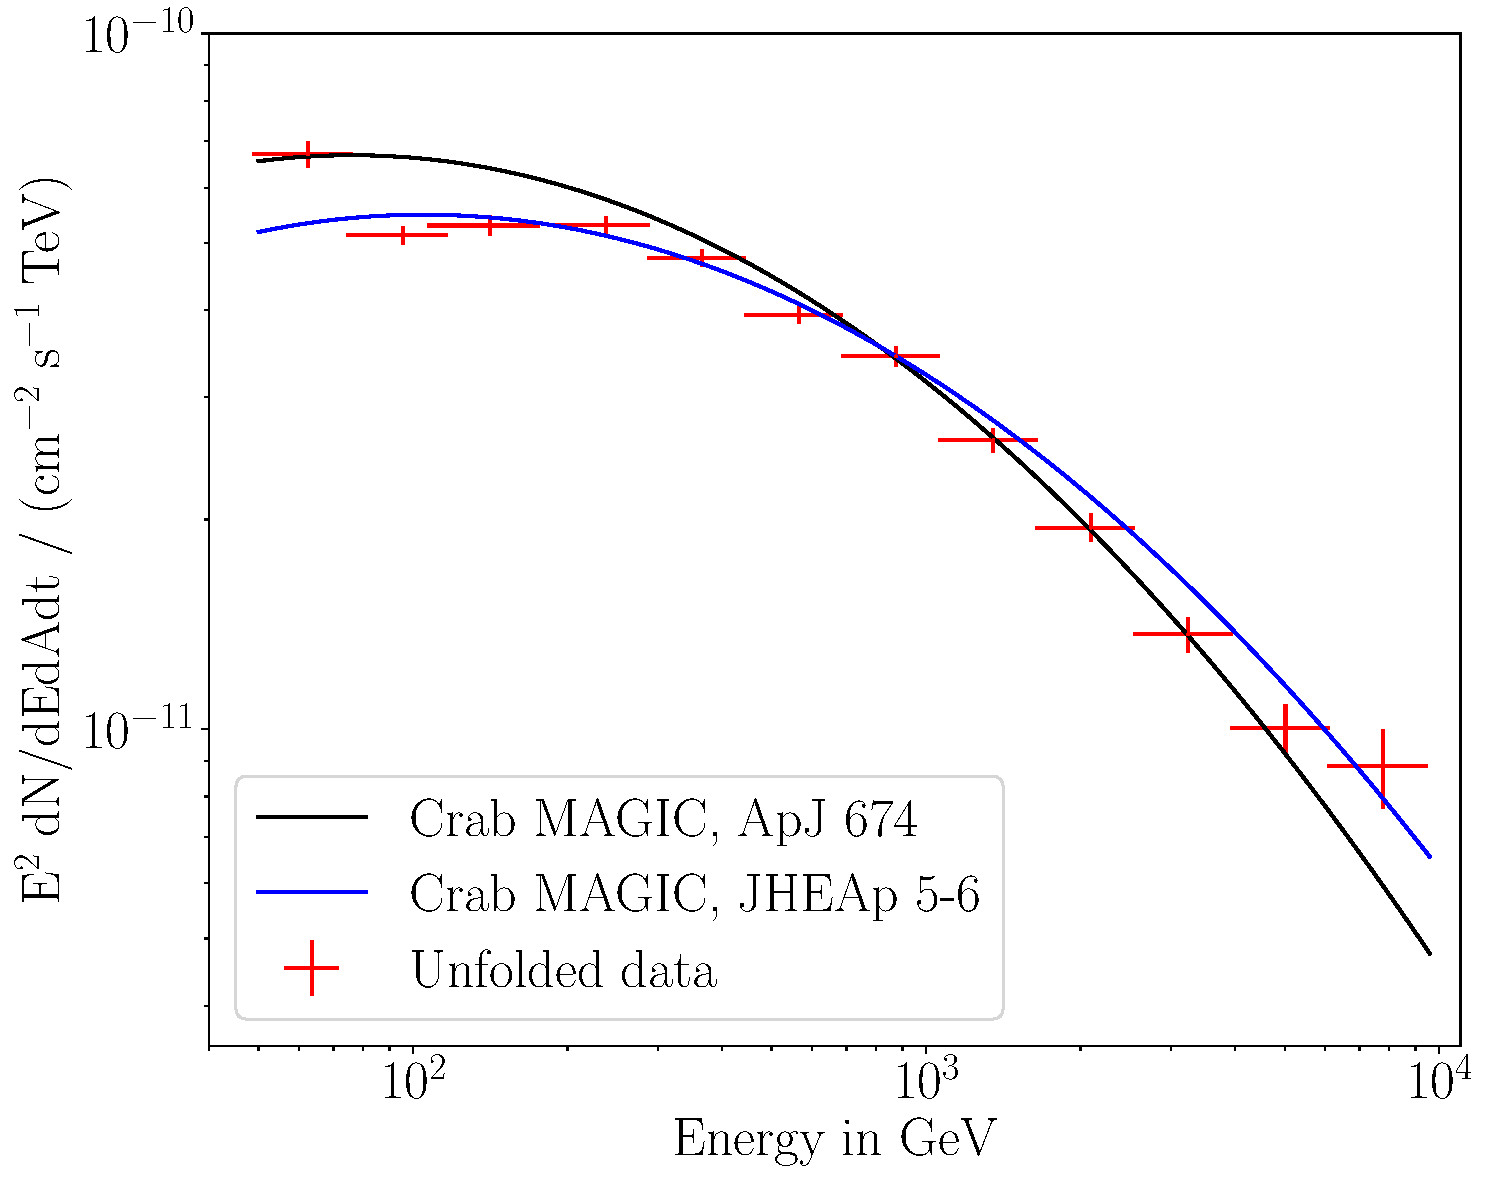
\includegraphics[width=0.8\textwidth]{figures/combunfold_energyspectrum.pdf}
  \caption{Entfaltetes Energiespektrum aufgetragen in Bins der Energie. Unter
  Berücksichtigung der statistischen Unsicherheiten sind die Messwerte
  kompatibel mit Referenzmessungen.}
  \label{fig:entfaltung}
\end{figure}
